\chapter{AMD GPU Internals} \label{chap:AMD_GPU_internal}
% AMD GPU 內部結構
雖然第2章介紹了編寫 HIP GPU 程式的基礎知識,但並未揭示如何調校效能。使用 GPU 加速器的動機是為了盡可能實現最佳化效能。因此,GPU 軟體工程師不應滿足於僅僅產生正確答案的實作。相反地,應該嘗試改進實作,以優化kernel函數的運行效能。在本章及下一章中,我們將討論幾種優化技術。本章涵蓋了與 GPU 硬體相關的重要概念,並為理解利用驚人硬體特性的高效能 GPU 程式設計技術奠定基礎。

GPU 的架構對程式效能有深遠的影響,優化通常包含利用特定的硬體機制(例如,memory coalescing)。本章首先簡要介紹支援 ROCm 和 HIP 的 AMD GPU。除非另有說明,否則討論的是 MI100 GPU \cite{amd2021cdna2}。

\section{AMD GPUs}
在深入探討架構細節之前,我們將檢視 AMD GPU 的演變,以加深理解。表6.1列出了幾款著名的 AMD GPU 產品。

現代 AMD GPU 架構可追溯到第一個 Graphics Core Next,簡稱 GCN,架構設計。GCN 是 AMD GPU 架構家族的名稱,首次發布於 2011 年,並使用至 2018 年。第一個 GCN GPU 是 AMD Radeon HD 7970。隨後,AMD 改進了該架構,創建了新改進的版本(即 GCN2 和 GCN3)。前三個 GCN 模型使用28奈米技術製造。然而,GCN4 和 GCN5 分別使用12奈米和14奈米技術製造(即 Polaris 和 Vega)。

AMD 使用「gfx」版本命名法,所有晶片版本均以「gfx」前綴開頭。每個版本的名稱由三個數字組成(即主版本號、副版本號和修訂號)。例如,MI100 GPU 使用 gfx908 晶片,其中「9」是主版本號,「0」是副版本號,「8」是修訂號。例如,Radeon RX 5700 XT 是第 10 代 AMD GPU;因此,其主版本號為 10。新的版本號通常表示新的、非向後兼容的指令集架構(ISA),而副版本和修訂則包含指令擴展和配置更改。

單晶片 AMD GPU 設計的多功能性在於其能夠透過細微修改和參數調整適應各種 GPU 產品。其中一個例子是 gfx803 晶片,它是至少五款不同 GPU 的基礎。它被用於 AMD 的高檔遊戲和計算 GPU(如 R9 Fury X、R9 Fury Nano)、中檔遊戲 GPU(如 Radeon RX 480、Radeon RX 580)以及計算專用 GPU(如 MI8)。

最近,隨著電晶體尺寸越來越小,AMD 開始專攻研究其 GPU 架構設計,針對不同的使用案例,將單一 GPU 架構拆分為兩種架構。

對於高效能通用計算,AMD 開發了 Compute DNA(CDNA)架構。雖然 CDNA 架構持續使用 gfx9 系列晶片,保持了 GCN 相同架構原則,但它引入了重大創新以增強計算效能並適應現代 workload 。CDNA GPU 的一個顯著特點是包含矩陣核心,旨在以更高的吞吐量執行矩陣乘法計算。在引入 CDNA 架構之後,AMD 推出了兩個新迭代版本:CDNA2 和 CDNA3。CDNA2 架構,以 MI210 和 MI250 GPU 為例,利用多晶片模組技術。這一進展大幅增加了每個 GPU 上的電晶體數量和計算資源,提供了更高的效能。此外,CDNA3 架構透過採用 3D 整合技術進一步推進了這一概念。這種方法包含垂直堆疊多個晶片,有效提高了電晶體密度和整體效能。

針對遊戲市場,AMD 開發了 RDNA 架構。RDNA 架構的重新設計是對 GCN 架構的重大革新,主要目的是減少延遲以提供更好的遊戲體驗。我們將在第6.10節中透過比較 GCN 和 CDNA 架構來介紹 RDNA 架構。

\begin{table}[htbp]
    \centering
    \caption{近期AMD GPU產品總整理}
    \label{tab:amd-gpu-summary}
    \begin{tabular}{@{}lllll@{}}
        \toprule
        \textbf{Release Date} & \textbf{Product Name}      & \textbf{Chip} & \textbf{Architecture} & \textbf{Transistor Size} \\ \midrule
        Dec. 2011            & Radeon HD 7970            & gfx600        & GCN                   & 28 nm                    \\
        Nov. 2013            & Radeon R9 290             & gfx701        & GCN2                  & 28 nm                    \\
        Jun. 2015            & R9 Fury X                 & gfx803        & GCN3                  & 28 nm                    \\
        Aug. 2015            & R9 Fury Nano              & gfx803        & GCN3                  & 28 nm                    \\
        Dec. 2016            & Radeon Instinct MI8       & gfx803        & GCN3                  & 28 nm                    \\
        Jun. 2016            & Radeon RX 480             & gfx803        & Polaris (GCN4)        & 14 nm                    \\
        Apr. 2017            & Radeon RX 580             & gfx803        & Polaris (GCN4)        & 14 nm                    \\
        Aug. 2017            & Radeon RX Vega 56         & gfx900        & Vega (GCN5)           & 14 nm                    \\
        Aug. 2017            & Radeon RX Vega 64         & gfx900        & Vega (GCN5)           & 14 nm                    \\
        Jun. 2017            & Radeon Instinct MI25      & gfx900        & Vega (GCN5)           & 14 nm                    \\
        Feb. 2019            & Radeon VII                & gfx906        & Vega (GCN5)           & 7 nm                     \\
        Jul. 2019            & Radeon RX 5700XT          & gfx1010       & RDNA                  & 7 nm                     \\
        Oct. 2020            & Radeon RX 6900XT          & gfx1030       & RDNA2                 & 7 nm                     \\
        Nov. 2020            & Instinct MI100            & gfx908        & CDNA                  & 7 nm                     \\
        Nov. 2022            & Instinct MI210/MI250      & gfx90a        & CDNA2                 & 7 nm                     \\
        Nov. 2022            & Radeon RX 7900 XTX        & gfx1100       & RDNA3                 & 5/6 nm                   \\
        Jan. 2023            & Instinct MI300            & gfx940        & CDNA3                 & 5 nm                     \\ \bottomrule
    \end{tabular}
\end{table}

\section{整體架構}
% 整體架構
GPU 由多個相互連接的blocks組成(不要與thread blocks混淆),這些block是相對獨立的數位電路,能夠完成預定的任務。有些是可程式化的,其他則執行固定的操作。它們協同工作,使 GPU 能夠執行複雜的程式和大規模的平行計算任務。在此,我們介紹對通用計算至關重要的 GPU blocks,並討論它們的組織架構(見圖6.1)。在本章稍後部分,我們將更詳細地討論每個block。

AMD GPU blocks主要分為三大組(控制、使用者可程式化的shader 和記憶體)。控制組包括指令處理器、非同步運算引擎(ACE)和直接記憶體存取(DMA),主要負責與 CPU 互動並控制shader和記憶體區塊。

\begin{figure}
    \centering
    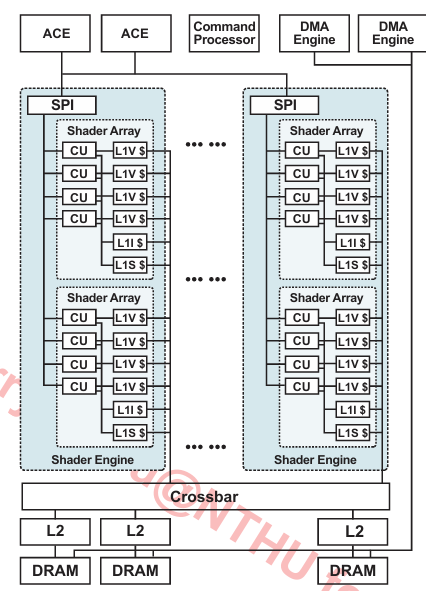
\includegraphics[width=0.5\linewidth]{FileAusiliari//Screenshots/Figure6-1.png}
    \caption{整體 AMD GCN GPU 架構。}
    \label{fig:enter-label}
\end{figure}

shader blocks被組織成三層的階層結構:shader engines、shader arrays和運算單元(CUs)。這種組織方式允許每一層的block共享不同的資源。例如,同一個shader array中的 CU 共享指令快取;而在同一個shader engine中的 CU 共享shader pipe input(SPI)block。這種組織方式實現了模組化的硬體設計,使 GPU 的配置可以輕鬆更改。例如,雖然 R9 Fury X 和 Radeon RX 480 GPU 都使用 gfx803 設計,但它們的配置不同。R9 Fury X 包含 16 個shader arrays,每個array有 4 個 CU,而 RX 480 GPU 包含 12 個shader arrays,每個array只有 3 個 CU。

最後,記憶體組包括 L2 快取,記憶體控制器透過data fabric設計連接,以支援一致性。它們共同儲存 GPU 計算所需的資料。這些 GPU 通常包含多組 L2 快取和記憶體控制器,提供對位址空間區段的讀取。GPU 的記憶體組可以平行工作,為 CU 提供大量的資料。

\section{指令處理器與 DMA 引擎}
% 指令處理器與 DMA 引擎
從前一章我們知道,GPU 必須在 CPU 的密切監督下執行計算任務。指令處理器是接收 CPU 命令的 GPU block(例如,記憶體複製和kernel啟動)。一般而言,指令處理器根據命令類型,將接收到的命令委派給其他 GPU block。例如,記憶體複製命令被轉發給 DMA 引擎,而kernel啟動命令被轉發給 ACE。

如果要將資料從 CPU 複製到 GPU,DMA 引擎會從 CPU 的系統記憶體中提取小區塊,並直接將它們儲存在其本地的動態隨機存取記憶體(DRAM)中。GPU 到 CPU 的記憶體複製則在相反方向上遵循類似的模式。DMA 引擎監督記憶體傳輸,但無法同時處理兩個記憶體複製命令。CPU 不直接參與記憶體複製過程,但負責初始化 DMA 引擎。

大多數 GPU 配備了兩個 DMA 引擎,因此可以在相同或相反的方向上同時處理兩個記憶體複製。擁有兩個 DMA 引擎可以更好地利用雙向的高速序列計算機擴充匯流排標準(PCIe)。

\section{ Workgroup Dispatching}

kernel啟動指令由非同步運算引擎(ACE)處理,ACE 將kernel拆分為workgroup,再分配給 SPI block,SPI block會進一步拆分為wavefront。

顧名思義,ACE 能夠同時且非同步地處理來自不同命令佇列或串流的指令。詳細內容請參見第4章。AMD GPU 配備了多個 ACE,可平行處理多個指令。ACE 亦允許同時執行多個kernel。雖然每個 ACE 一次只能 dispatch 一個kernel,但擁有多個 ACE 的 GPU 可以同時執行多個kernel。我們在第4.2.4節討論了同時執行多個kernel的折衷方法。

SPI 負責將wavefronts dispatch 到運算單元(CU),並初始化registers,使得wavefront指令能夠以必要的參數執行。SPI 保證同一workgroup內的所有wavefronts都 dispatch 到相同的 CU,以便它們能夠同步。

在 CU 中執行wavefront會消耗資源,當資源耗盡時,wavefront會排隊等待活躍的wavefront完成。CU 消耗四種資源類型:wavefront slots、純量通用型暫存器(SGPRs)、向量通用型暫存器(VGPRs)以及本地資料共享(LDS)。我們將在本章後面討論結構時詳細介紹這些。

kernel擁有的workgroup數量通常超過 GPU 同時能執行的數量。因此,ACE 單元會在活躍workgroup完成執行時 dispatch 新的workgroup。由於並非所有workgroup都能同時執行,GPU 無法同步單一kernel中的所有work items。考慮 Listing 6.1 的範例,kernel中的每個thread執行任務的第一步並將計數器加一。然後,每個kernel等待計數器達到其thread總數,這表示第一步已完成。接著,所有thread進入第二步。kernel是否能完成執行取決於其workgroup數量與 GPU 同時執行數量之間的關係。如果 GPU 能夠同時在所有 CU 上運行 64 個workgroup,且派遣的workgroup數量小於 64,kernel將執行它們。然而,如果workgroup數量超過 64,kernel將在迴圈中發生deadlock,因為只有前 64 個workgroup能在 CU 上執行,其餘的workgroup將不會被排程。因此,計數器永遠無法達到適當的 \texttt{num\_thread\_in\_kernel} 水準,導致不可恢復的 deadlock。

%"mystyle" code listing set
\lstset{style=mystyle}
%  Listing 6.1:deadlock範例程式碼。計數器定義為一個volatile指標,並初始化為零。
\begin{lstlisting}[language=c++,caption={deadlock範例程式碼。計數器定義為一個volatile指標,並初始化為零。}]
// 執行步驟 1。

atomicInc(counter);
while (true) {
    if (*counter >= num_thread_in_kernel) {
        break;
    }
}

// 執行步驟 2。
\end{lstlisting}

Workgroup與 CU 的映射是非確定性的。ACE 和 SPI 根據每個 CU 可用的資源將workgroup指派到 CU。即使以相同的參數執行kernel兩次,也不一定會將workgroup指派到相同的 CU。因此,程式設計師不能假設特定的workgroup與 CU 的映射,也不應嘗試根據workgroup執行的位置來提升效能。

\section{Sequencer}
\label{sec:sequencer}
\begin{figure}[h]
    \centering
    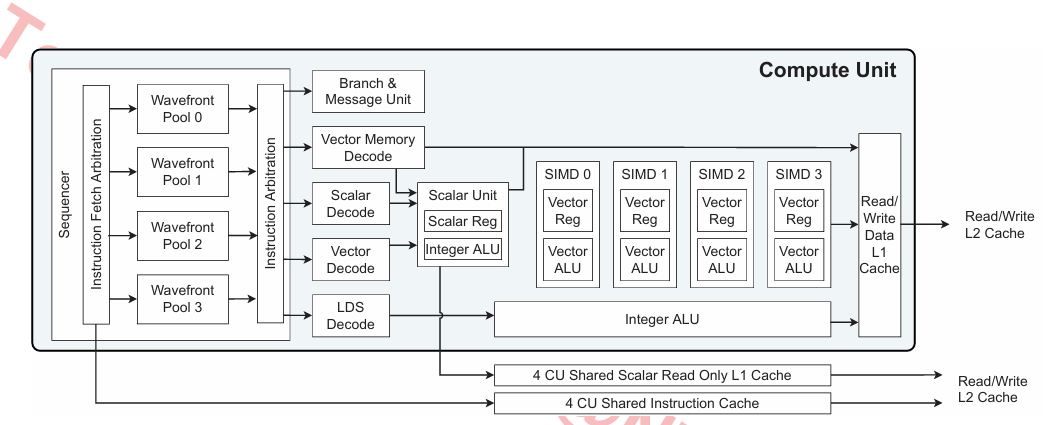
\includegraphics[width=1\linewidth]{FileAusiliari//Screenshots/Figure6-2.png}
    \caption{CU 架構(感謝 AMD 提供)。}
    \label{fig:enter-label}
\end{figure}

一個 GPU 的 CU 可以進一步細分為子區塊(見圖6.2)。在本節中,我們將通過追蹤指令如何通過子區塊來描述 CU 的組織結構。

CU 的核心是 instruction sequencer block(SQ),負責向執行單元 issue 指令。SQ 持有一個wavefronts及其指令的 列表。這個列表被組織成四個pools,每個pool包含 10 個 wavefront slots。一個slot包括托管 wavefront所需的硬體資源,包括wavefront-level registers(例如,程式計數器)和指令緩衝區。因此,理論上,一個 CU 最多可以同時執行 40 個wavefronts。

\textbf{指令讀取( Instruction-fetching)}。要執行一個指令,首先必須從記憶體中讀取。為了確定哪個wavefront可以讀取指令,SQ 配備了一個讀取仲裁器。在每個週期中,讀取仲裁器從等待中的wavefronts中選擇最早 dispatch 的wavefront。因此,一個 CU 每個週期可以讀取 32 位元組的指令(總共 4 至 8 條),因為每條指令的大小為 4 至 8 位元組。


\textbf{Instruction-issuing}。讀取到的指令必須 issue 到執行單元。因此,SQ 配備了一個 issue 仲裁器,決定每個週期可以 issue 的指令。

注意,指令總是在wavefront級別 issue 。執行單元運行wavefront中所有work items的指令。因此,work items實際上是同步執行的,確保它們在特定時間執行相同的指令。

每個 CU 根據指令類別(例如,純量、分支、向量、向量記憶體和 LDS)擁有不同的執行單元。這在不同指令類型可以平行執行方面具有優勢。指令的類型在其二進位碼中編碼,以便仲裁器能夠識別將其dispatch 到哪裡。

在每個週期中, issue 仲裁器從四個pools中的一個選擇wavefront。因此, issue 仲裁器最多可以從 10 個wavefronts中選擇。只要滿足以下兩個條件,單個週期中可以有多個wavefronts issue 指令。首先,wavefront不得 issue 佔用相同執行單元的指令。這很直觀,因為執行單元一次只能處理一個指令。其次,如果wavefront已經在執行一個指令,則不應 issue 另一個指令。這簡化了sequencer的設計,因為它不需要考慮複雜的暫存器依賴性。 issue 仲裁器在每個週期後按照round-robin 模式切換wavefront pools。

GPU 的指令管線設計與典型的 CPU 有著顯著的差異。在 CPU 中,管線中執行的指令通常來自同一個thread。然而,由於 GPU 依賴於thread層級的平行處理,不同wavefronts中的指令可以在管線的不同階段執行。

一個經常被忽略的 GPU 執行特性是,每當切換到另一個work item或wavefront時,GPU 都會發生 context-switching 。然而,由於這種切換在每個週期內進行,因此不會產生任何額外的切換開銷。

\section{SIMD Unit}
SIMD 單元是提供 GPU 大部分計算能力的區塊。它們負責執行 SQ  dispatch 的向量指令,每個 SIMD 單元包含一組算術邏輯單元(ALUs),可以對特定數據類型進行計算操作。通常,一個 SIMD 單元擁有 16 個單精度 ALUs。在每個週期中,SIMD 單元執行來自 16 個work items的其中一條指令。考慮到每個wavefront包含 64 個work items,一個 SIMD 單元需要四個週期才能執行一條指令。

\begin{figure}
    \centering
    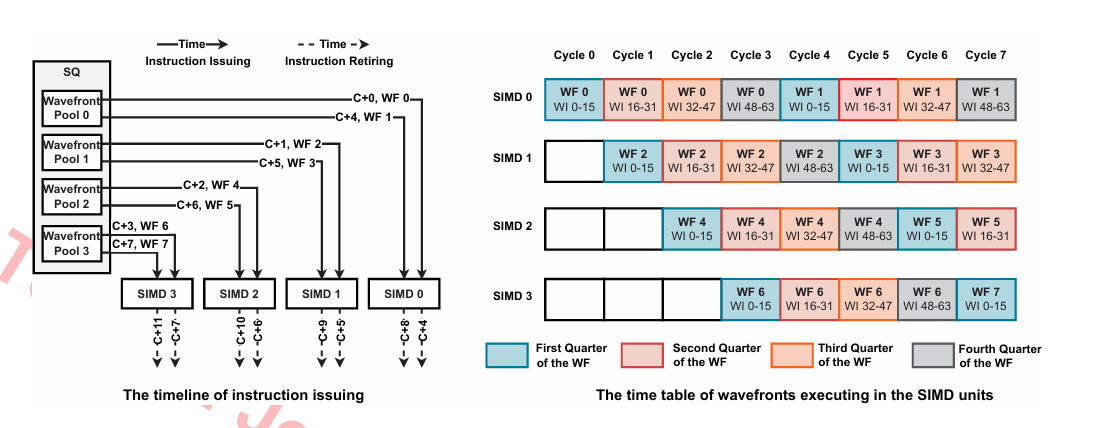
\includegraphics[width=1\linewidth]{FileAusiliari//Screenshots/Figure6-3.png}
    \caption{向 SIMD 單元 issue 指令的時序。}
    \label{fig:enter-label}
\end{figure}

如圖6.3所示,wavefront pools和 SIMD 單元之間存在一對一的映射。來自一個pool的wavefront只能 issue 到其對應的 SIMD 單元。這並非巧合,因為 SIMD 單元數量與執行一個wavefront指令所需的週期數相匹配。如果一條向量指令在週期 C+0 被 issue ,SIMD 單元會在 C+1 到 C+4 週期內執行它。由於有四個wavefront pools, issue 仲裁器需要四個週期才能有機會再次從同一pool中 issue 另一條指令。因此,在週期 C+4,另一條指令可以被 issue 並在週期 C+5 開始執行。這種設計確保了如果有足夠數量的 SIMD 指令等待執行,SIMD 單元可以被充分利用。

我們可以根據 SIMD 單元的數量來估計其理論計算吞吐量。因為每個 MI100 GPU 擁有 120 個 CU,每個 CU 包含四個 SIMD 單元,每個 SIMD 單元包含 16 個單精度 ALU 單元。因此,每個 GPU 每個週期可以執行 120×4×16 = 7,680 條單精度指令(IPC)。如果將這個數字乘以 MI100 CU 的時鐘頻率 1,502 MHz,我們發現這個 GPU 每秒可以執行約 $7,680 \times 1,502 \times 10^6 \approx 11.5 \times 10^{12}$
 條單精度指令。最後,由於每條指令可以在fused multiply–add register (FMA) 中編碼兩個操作,理論計算能力高達每秒約 $11.5 \times 10^{12} \times 2 \approx 23$ 單精度兆浮點運算(TFLOPS)。

 \section{Thread Divergence}
 理想情況下,wavefront的指令執行將為組成wavefront的所有64個work items產生結果。然而,實際上thread divergence 是不可避免的,以下是一個簡單的範例,展示在以下 kernel 程式碼中,32個work items必須執行第2行,另32個work items必須執行第4行:
 %"mystyle" code listing set
\lstset{style=mystyle}
%  Listing 6.2:diverging範例程式碼。
\begin{lstlisting}[language=c++,caption={diverging範例程式碼。}]
if (thread_id < 32) {
    a = a + 1;
} else {
    a = a + 2;
}
\end{lstlisting}

由於 GPU 的指令是以wavefront granularity issue ,因此無法為部分work items issue 範例中第2行的指令時,同時為其他work items issue 第4行的指令。第2行執行的指令必須為wavefront中的所有64個work items執行。為避免產生不正確的結果,每個wavefront都關聯一個64位元的執行遮罩暫存器。遮罩中的每一位元表示每個work item的結果將如何被更新。例如,在第1行,執行遮罩被設置為16進位值0x0000,0000,ffff,ffff,表示僅在執行第2行時會更新(即committed)與下32個work items相關的結果。ELSE語句會翻轉執行遮罩,將其改為0xffff,ffff,0000,0000,允許在執行第4行時生效上32個work items。最後,執行遮罩被重置為0xffff,ffff,ffff,ffff,以便所有work items執行kernel的剩餘部分。預測(Predication)是使用遮罩來決定哪些指令可以生效的過程。值得注意的是,GPU的預測執行會導致thread divergence,意味著wavefront中的thread會遵循不同條件分支。

請注意,IPC是CPU常用的性能評估指標。然而,為了分析GPU效能,有必要澄清所報告的指令層級。預測略微複雜化效能分析。一般來說,程序員會使用wavefront級和work item級的指令。wavefront級的指令計數不考慮執行遮罩的狀態,而work item級的指令計數僅累加由執行遮罩標記為有效的work items。假設執行遮罩為0xffff,ffff,ffff,ffff,且所有指令都是由SIMD單元處理的向量ALU類型,則CU應該產生wavefront級IPC為1,work item級IPC為64。

根據我們對 Listing 6.2中程式碼片段的分析,第2行和第4行無法同時執行。此外,儘管只有一半的work items會在第2行和第4行產生結果,但執行所有向量指令仍需四個SIMD單元週期。也就是說,在沒有分支的情況下,一個SIMD執行64個work items級指令需要四個週期。在 Listing 6.2的範例中,執行64個work items級指令至少需要八個週期。在這種情況下,儘管CU的wavefront級IPC仍為1,work item級IPC則減少到32。最糟糕的情況是每個thread執行不同的分支。在這種情況下,執行64個work items級指令將需要$64 \times 4 = 256$個週期,導致work item級IPC減少到1。因此,應盡可能避免thread divergence。

\section{Memory Coalescing} \label{sec:memory_coalescing}
GPU被設計來高效處理資料。然而,在開始處理之前,資料必須從GPU記憶體中讀取並傳送到每個CU。
稍後,結果將寫回到GPU記憶體中。AMD的CU依賴特殊的載入和儲存指令來分別從GPU記憶體讀取和寫入資料。這些指令所產生的記憶體 transactions 由texture-addressing(TA)區塊處理。

GPU的載入和儲存指令在記憶體中是向量化的。對於一條wavefront級指令,每個work item將有自己的位址和資料。然而,兩個work items同時讀取和寫入同一記憶體位址是很常見的。更常見的是,work items可能讀取相鄰的資料項目或位於鄰近的資料項目。在這種情況下,這兩個資料項目可以通過單一的記憶體 transaction(通常為64位元組)來讀取。因此,TA區塊可以合併部分work item的記憶體讀取,從而減少記憶體 transaction 數量。這一重要機制稱為memory coalescing。

圖6.4中的範例程式碼將矩陣資料載入CU暫存器,說明了memory coalescing。如果我們有一個1024 × 1024的單精度矩陣,儲存在GPU記憶體中,並以行column主序(即連續位址位於相鄰行中)排列,且起始位址為零,我們可以假設有兩種選擇:我們可以垂直載入,按列逐列讀取資料,或者水平載入,按行逐行讀取資料。當垂直載入時,第一個work item讀取位址0,第二個讀取位址4096,第三個讀取位址8192,依此類推。這樣,TA區塊無法合併記憶體讀取,必須為單一wavefront issue 64個記憶體 transaction 。我們將這種記憶體讀取模式稱為non-coalescable,它會顯著影響效能。

\begin{figure}
    \centering
    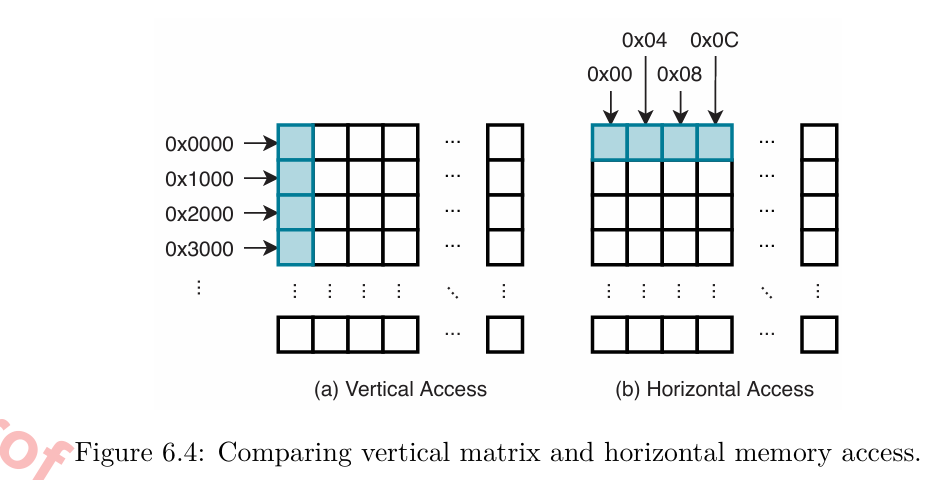
\includegraphics[width=1\linewidth]{FileAusiliari//Screenshots/Figure6-4.png}
    \caption{比較垂直矩陣和水平記憶體存取}
    \label{fig:enter-label}
\end{figure}

相反,我們可以水平存取跨行的資料。第一個work item讀取位址0,第二個讀取位址4,第三個讀取位址8,依此類推。在這種情況下,wavefront中的64個work items要讀取的記憶體是一個256位元組的連續位址區塊。因此,如果記憶體讀取granularity為64位元組,TA區塊可以將交易數量減少到僅四次讀取:相比垂直排列,記憶體 transaction 數量僅為6\%。我們將這種類型的讀取模式稱為coalescable。

Memory coalescing相比於non-coalesced讀取模式提供了主要的效能優勢,因為後者會浪費寶貴的記憶體頻寬。因此,應盡可能使用連續讀取模式。稍後在第8.5節,我們將探討更多將不連續讀取轉換為連續讀取的軟體解決方法。

\section{Memory Hierarchy}
在 kernel 開始執行之前,資料會被儲存在 GPU 的記憶體中。GPU 通常配備 DRAM 記憶體單元,如圖形用雙倍數據傳輸率存儲器(GDDR)或高頻寬記憶體(HBM)類型的 DRAM。一般來說,GDDR 的讀取延遲較低,而 HBM 則提供更高的頻寬。由於大數據處理應用程式高度依賴記憶體且對頻寬敏感,HBM 更適合用於通用計算。HBM 被用於 MI100 GPU 上。


運算單元(CUs)必須在計算之前,將資料從 GPU 記憶體轉移到本地暫存器。通常,使用 GDDR 還是 HBM 並不重要,因為延遲和頻寬無法滿足確保 SIMD 單元全速運行的需求。為了減少延遲並提升頻寬,CUs 與 DRAM 之間提供了兩級快取,使用靜態隨機存取記憶體技術(SRAM),其反應速度遠快於 DRAM,並能提供更高的頻寬。

\begin{figure}
    \centering
    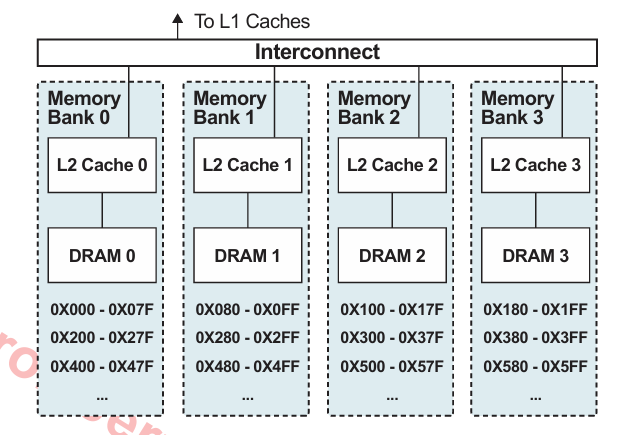
\includegraphics[width=1\linewidth]{FileAusiliari//Screenshots/Figure6-5.png}
    \caption{GPU memory bank組織}
    \label{fig:enter-label}
\end{figure}

作為 L1 快取,每個 CU 專屬一個每管道的紋理快取(TCP)區塊。L1 快取是write-through快取,意味著所有寫入 L1 快取的資料也會直接寫入 L2 快取。


AMD GPU 的 L2 快取(即texture cache channel(TCC)區塊)是記憶體側快取。如圖6.5所示,每個 L2 快取都連接到一個 DRAM 控制器,L2 群組和記憶體控制器形成一個memory bank,不要與以更細微度運作的 DRAM banks混淆。memory bank覆蓋固定範圍的記憶體位址,通常以128位元組的維度交錯排列。交錯排列允許memory bank同時讀寫,從而提高有效記憶體頻寬。

支援快取一致性是多核心 CPU 設計中的一個主要考量。如果不維持快取一致性,多thread執行可能會產生不正確的結果。例如,如圖6.6所示,一個資料項目(由資料位址識別)可以同時存在於三個快取中。如果Core 1寫入該資料,只有本地的 L1 快取會被更新,其他 L1 和 L2 快取中的資料則會過時。未來核Core 2的讀取將無法取得Core 1更新後的資料。對於 CPU,常見的解決方案是引入快取一致性協議,在寫入之前從其他 L1 快取中移除該cache line。

\begin{figure}
    \centering
    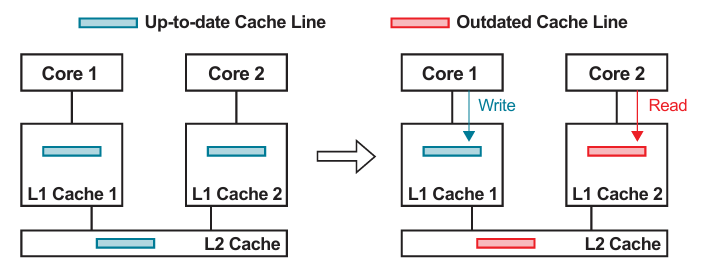
\includegraphics[width=1\linewidth]{FileAusiliari//Screenshots/Figure6-6.png}
    \caption{多核心 CPU 中快取一致性問題範例}
    \label{fig:enter-label}
\end{figure}
\begin{figure}
    \centering
    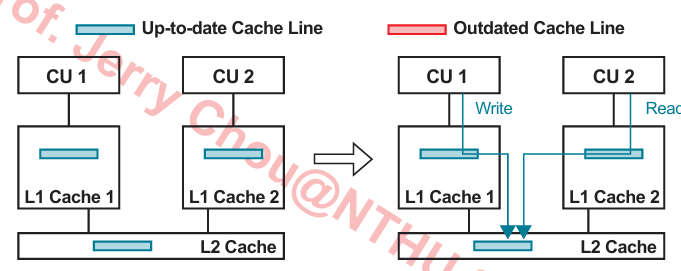
\includegraphics[width=1\linewidth]{FileAusiliari//Screenshots/Figure6-7.png}
    \caption{GPU 一致性支援使用write-through L1 快取}
    \label{fig:enter-label}
\end{figure}

GPU 的快取一致性支援較為簡單。由於每個存取指令同時寫入 L1 和 L2 快取,L2 快取始終保持最新版本。使用write-through的 L1 快取就不需要添加複雜且會影響效能的一致性協議。

有讀者可能會問,如果一個cache line存在於兩個 L1 快取中,且一個 CU 在另一個 CU 讀取之前寫入會發生什麼情況(見圖6.6)。儘管 GPU 的write-through L1 快取可以更新 L2 中的資料,但其他 L1 快取中的cache lines不會被無效化或更新。一般而言,從一個thread寫入資料並從另一個thread讀取更新後的版本在 GPU 程式設計中並不受支援。如果需要這種同步,程式設計師必須使用全域記憶體屏障或atomic operations。另一個選擇是使用兩個 kernel 來分開讀取和寫入。

AMD GPU 在 L2 快取中執行atomic operations。當一個 CU 執行atomic instruction時,該指令會被送到 L2,並在本地儲存中處理。雖然 GPU 不需要一致性協議,但我們仍須考慮當兩個 CUs 同時寫入同一cache line的不同部分時(「假共享」)會發生什麼。如果設計不當,第二次寫入將會覆蓋 L2 中的第一次寫入。為避免這種情況,AMD GPU 使用基於寫遮罩的設計,每個記憶體寫入請求時,CUs 和 L1 快取會使用位元來表示應該更新 L2 快取中的哪一組位元組,並發送寫入(「dirty mask」)。每個cache line的每4位元組會提供一個位元。因此,使用這種方法,兩次寫入可以輕鬆地在 L2 快取中合併,允許 CUs 平行寫入,同時維持正確性並提升整體記憶體吞吐量。

\section{AMD RDNA GPUs}

AMD RDNA 架構是基於 GCN 架構的自然演進,主要針對下一代高效能遊戲而量身打造。它引入了顯著的核心和記憶體架構設計修改,以提升可擴展性和效率。雖然主要針對遊戲 workload ,配備 RDNA 的 GPU 具備高效能的計算核心,也適用於通用計算。自 ROCm 6.0 版本起,支援五款 RDNA GPU 產品:Radeon RX 7900 XTX、Radeon RX 7900 XT、Radeon Pro W7900、Radeon Pro W6800 和 Radeon Pro V620。

GCN 與 RDNA 架構的主要區別在於其wavefront大小。GCN 使用 64 個work items的wavefront,而 RDNA 將此數量減少到 32 個work items。這一變更旨在改善 CU 處理現代 workload 中的thread divergence問題。較小的wavefront大小也設計用來降低載入/儲存指令所產生的記憶體 transaction 數量,目的是減少記憶體讀取延遲並提高 ALU 使用率。然而,為了向下兼容,RDNA GPU 在兼容模式下支援 64 work items的wavefront。是否將 kernel 編譯為 32 或 64 work items模式由編譯器決定。

RDNA GPU 的一個顯著變化是引入了Dual Compute Units (DCUs),取代了 CDNA 的運算單元(CUs)。每個 DCU 包含四個排程器,負責讀取和 issue 指令,這相較於 CDNA CU 中的單一排程器有了大幅提升。這一改進提升了指令 issue 機率。與 GCN 架構中一個排程器向四個 SIMD 單元發出指令不同,RDNA 排程器僅負責一個 SIMD 單元。每個 SIMD 單元包含 32 個單精度 ALU,並以較窄的 32 work items wavefront運行,因此 DCU 的 SIMD 單元可以在每個週期執行一條指令,這相比 GCN CU 中每條指令需四個週期的執行時間有了顯著改善。此外,每個 DCU 擁有雙倍於單一 CU 的計算資源,並包含一個統一的本地資料共享單元。

RDNA 架構透過實施包含 L0、L1 和 L2 快取的三級快取結構,徹底改變了快取層級。RDNA 的 L0 快取對應於 GCN 架構中的 L1 快取,因為它們直接連接到 DCU,並專屬於每個 DCU。此外,RDNA 引入了一個位於 L0 和 L2 快取之間的中間 L1 快取。此 L1 快取服務於一組 DCU(通常在大多數硬體配置中有五個)。其作用是減少對 L2 快取的請求頻率,從而降低晶片間的資料流量。這一優化提升了效能並降低了功耗。

RDNA 的快取設計另一個重要變更是將 L0 向量快取、L1 快取和 L2 快取的cache line大小從 64 位元組增加到 128 位元組。這一增加具有策略意義,方便為wavefront中的 32 個work items傳送一組獨特的單精度數字,因為 4 位元組乘以 32 個work items等於 128 位元組。這一增強與架構強調的效率和效能優化相符。

這些 RDNA 架構的修改主要目標是通過最小化延遲來優化遊戲和圖形 workload ,而非最大化吞吐量。例如,能夠在每個週期處理一個wavefront指令減少處理延遲,確保更快交付結果。然而,這一改變並不一定提升整體計算能力。因此,針對不同應用領域的 CDNA 架構並未採用這些 RDNA 特有的變更。相反,CDNA 架構保留了更多與傳統 GCN 風格相符的設計特徵,專注於其預期使用案例相關方面。

\section{結論}
在本章中,我們了解 GPU 的硬體架構。對於 GPU 程式設計師而言,對 GPU 硬體運作有基本的理解至關重要,特別是如果他們希望在這些裝置上獲得最佳效能。這些知識將使他們能夠優化程式碼,充分利用 GPU 的平行運算硬體。此外,了解硬體中存在的基本特性有助於程式設計師開發無錯的平行程式。
